
\section{Estimation}

\subsection{Calibration}

I carry out the calibration using known parameters and steady-state targets. A first block of steady-state values and parameters is tractable.

\begin{align*}
\phi &= \frac{\epsilon - 1}{\epsilon}\\
u &= 1-n\\
n^f &= n \left( \frac{n^f}{n} \right)\\
n^p &= n-n^f\\
s &= \xi\left(\frac{s}{\xi}\right)\\
\delta &= \frac{\left( 1 - \left( \frac{n^f}{n} \right) \right) \left( \frac{\mu^f}{\mu^p+\mu^f}\right)}{\left( \frac{n^f}{n} \right) \left( 1-\left( \frac{\mu^f}{\mu^p+\mu^f}\right)\right)} \xi\\
e &= u+\delta n^f + \xi n^p\\
\mu^p &= \frac{\xi n^p}{e}\\
\mu^f &= \frac{\delta n^f}{e}\\
\end{align*}

Knowing $\xi$, $s$ and $\sigma^z$, it is possible to numerically solve for $z^p$ using the fact that $\xi = s + (1-s) G\left( z^p \right)$. Then, the following system in $\left( \overline{w^p}, U, F \right)$ --- where $U = b + \frac{\eta \gamma \theta}{1-\eta}$ --- is tractable.

\begin{align*}
&\overline{w^p} = \eta \phi \mathbb{E} \left[ z \mid z \geq z^p \right] + \eta (1-\beta(1-s)) F + (1-\eta) U \\
&\phi z^p + \left( 1 - \beta (1-s) \right) F + (1-s)  \beta \phi \int_{z^p}^{+\infty} \left( 1 - G(z) \right) dz = U \\
&F = \rho^F \overline{w^p} 
\end{align*}

Combining these three expressions, I get

\begin{align*}
&F = \frac{\rho^F \phi}{1 - \rho^F (1 - \beta (1-s))} \left( \eta \mathbb{E} \left[ z \mid z \geq z^p \right] + (1-\eta) \left( z^p + \beta (1-s) \int_{z^p}^{+\infty} \left( 1 - G(z) \right) dz \right) \right)\\
&U = \phi z^p + \left( 1 - \beta (1-s) \right) F + (1-s)  \beta \phi \int_{z^p}^{+\infty} \left( 1 - G(z) \right) dz
\end{align*}

It is possible to compute $z^c$.

\begin{align*}
&z^c = z^p + \frac{F}{\phi}\\
\end{align*} 

A non-linear system in $\left(z^f, z^*, \rho\right)$ can then be solved numerically.

\begin{align*}
&\rho z^f \phi + \rho \mathbb{E}_t \beta (1-\delta) \phi \left( \mathbb{E}z - z^f \right) = U \\
&(1-\rho) z^* = z^c - \rho z^f\\
&\frac{\mu^f}{\mu^p + \mu^f} = \frac{ G \left( z^*\right) - G \left( z^f\right) }{ 1 - G \left( z^f\right) }
\end{align*}

Then, one can derive $\left(\theta, \gamma, b, m \right)$.

\begin{align*}
&p = \frac{\mu^p}{1-G\left( z^*\right)}\\
&\theta = \frac{p}{q}\\
&\gamma = (1-\eta) \phi q \left( \int_{z^*}^{+\infty} \left( 1 - G(z) \right) dz + \rho \int_{z^f}^{z^*} \left( 1 - G(z) \right) dz \right)\\
&b = U - \frac{\eta \gamma \theta}{1-\eta} \\
&m = q \theta^{\sigma}\\
\end{align*}

Average wages of open-ended and fixed-term workers $w^p$ and $w^f$ write

\begin{align*}
w^p &= \eta \phi \left( (1-\xi) \mathbb{E} \left[ z \mid z \geq z^p \right] + \xi \mathbb{E} \left[ z \mid z \geq z^* \right]\right) + \eta \left( (1-\xi) F - \eta \beta (1-s) F \right) + (1-\eta) U\\
w^f &= \eta \phi \rho \left( (1-\delta) \mathbb{E} z + \delta \mathbb{E} \left[ z \mid z^f \geq z \geq z^* \right] \right) + (1-\eta) U\\
\end{align*}

Consequently, the average wage for all workers is

\begin{align*}
w = \frac{n^f}{n} w^f + \frac{n^p}{n} w^p
\end{align*}

$h$ verifies

\begin{align*}
h = \rho^b w - b 
\end{align*}

The parameters $\left( F, h, s, \delta, \rho, m, \gamma \right)$ are all determined at this point

\subsection{Data}

\begin{table}[H]
\begin{center}
\begin{tabular}{lll}
\toprule
Observable & Time range & Unique Identifier\\
\midrule
GDP at constant prices & 1995:Q1 - 2019:Q3 & \href{https://sdw.ecb.europa.eu/browseTable.do?node=qview&SERIES_KEY=320.MNA.Q.Y.I8.W2.S1.S1.B.B1GQ._Z._Z._Z.EUR.LR.N&trans=N}{MNA.Q.Y.I8.W2.S1.S1.B.B1GQ.\_Z.\_Z.\_Z.EUR.LR.N}\\
GDP deflator & 1995:Q2 - 2019:Q2 & \href{https://sdw.ecb.europa.eu/quickview.do?SERIES_KEY=320.MNA.Q.Y.I8.W2.S1.S1.B.B1GQ._Z._Z._Z.IX.D.N}{MNA.Q.Y.I8.W2.S1.S1.B.B1GQ.\_Z.\_Z.\_Z.IX.D.N}\\
Nominal interest rates & 1994:Q1 - 2019:Q3 & \href{https://sdw.ecb.europa.eu/quickview.do?SERIES_KEY=143.FM.M.U2.EUR.4F.MM.EONIA.HSTA&start=&end=&submitOptions.x=0&submitOptions.y=0&trans=QF}{FM.M.U2.EUR.4F.MM.EONIA.HSTA}\\
Employment & 1995:Q1 - 2019:Q3 & \href{https://sdw.ecb.europa.eu/browseChart.do?node=qview&SERIES_KEY=390.ENA.Q.Y.I8.W2.S1.S1._Z.EMP._Z._T._Z.PS._Z.N}{ENA.Q.Y.I8.W2.S1.S1.\_Z.EMP.\_Z.\_T.\_Z.PS.\_Z.N}\\
\bottomrule
\end{tabular}
\label{est_series}
\caption{Times series used for estimation}
\end{center}
\begin{flushleft}
\small All these time series are drawn from the ECB Data Warehouse
\end{flushleft}
\end{table}

\begin{table}[H]
\begin{center}
\begin{tabular}{p{2.5cm}llll}
\toprule
Observable & Symbol & Time range & Source & Unique Identifier\\
\midrule
Open-ended job creations & $jc^p$ & 2000:Q1 - 2019:Q3 & \href{https://www.acoss.fr}{Acoss} &  \href{https://www.acoss.fr/home/observatoire-economique/publications/acoss-stat/2019/acoss-stat-n296.html}{Acoss Stat 296}\\
Fixed-term job creations & $jc^f$ & 2000:Q1 - 2019:Q3 & \href{https://www.acoss.fr}{Acoss} &  \href{https://www.acoss.fr/home/observatoire-economique/publications/acoss-stat/2019/acoss-stat-n296.html}{Acoss Stat 296}\\
Share of fixed-term contracts in job creation & $\mu^f / \left( \mu^p + \mu^f \right)$ & 2000:Q1 - 2019:Q3 & \href{https://www.acoss.fr}{Acoss} &  \href{https://www.acoss.fr/home/observatoire-economique/publications/acoss-stat/2019/acoss-stat-n296.html}{Acoss Stat 296}\\
Share of fixed-term employment & $n^f$ &  2003:Q1 - 2019:Q3 & \href{https://www.insee.fr/}{Insee} & \href{https://www.insee.fr/fr/statistiques/serie/010605905}{010605905}\\
Endogenous open-ended job destruction & $jd^p$ & 2001:Q1 - 2017:Q4 & \href{https://dares.travail-emploi.gouv.fr/}{DARES} & \href{https://dares.travail-emploi.gouv.fr/dares-etudes-et-statistiques/statistiques-de-a-a-z/article/les-mouvements-de-main-d-oeuvre}{DMMO - EMMO}\\
Fixed-term job destruction & $jd^f$ & 1998:Q1 - 2017-Q4 & \href{https://dares.travail-emploi.gouv.fr/}{DARES} & \href{https://dares.travail-emploi.gouv.fr/dares-etudes-et-statistiques/statistiques-de-a-a-z/article/les-mouvements-de-main-d-oeuvre}{DMMO - EMMO}\\
Vacancies & $v$ & 1989:Q1 - 2019:Q2 & \href{http://www.oecd.org/}{OECD} & \href{https://fred.stlouisfed.org/series/LMJVTTNVFRQ647S}{LMJVTTNVFRQ647S}\\
\bottomrule
\end{tabular}
\caption{Labor market times series}
\end{center}
\end{table}

\subsection{Additional Graphs}

\begin{figure}[H]
\begin{center}
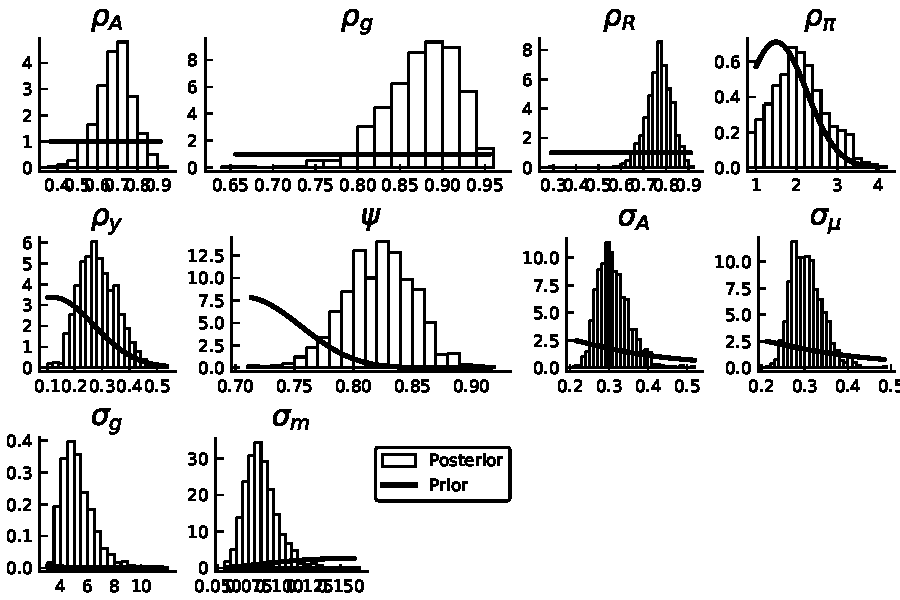
\includegraphics[scale=1]{prior_post.pdf}
\caption{Prior and posterior distributions}
\end{center}
\end{figure}

\begin{landscape}
\begin{figure}[H]
\begin{center}
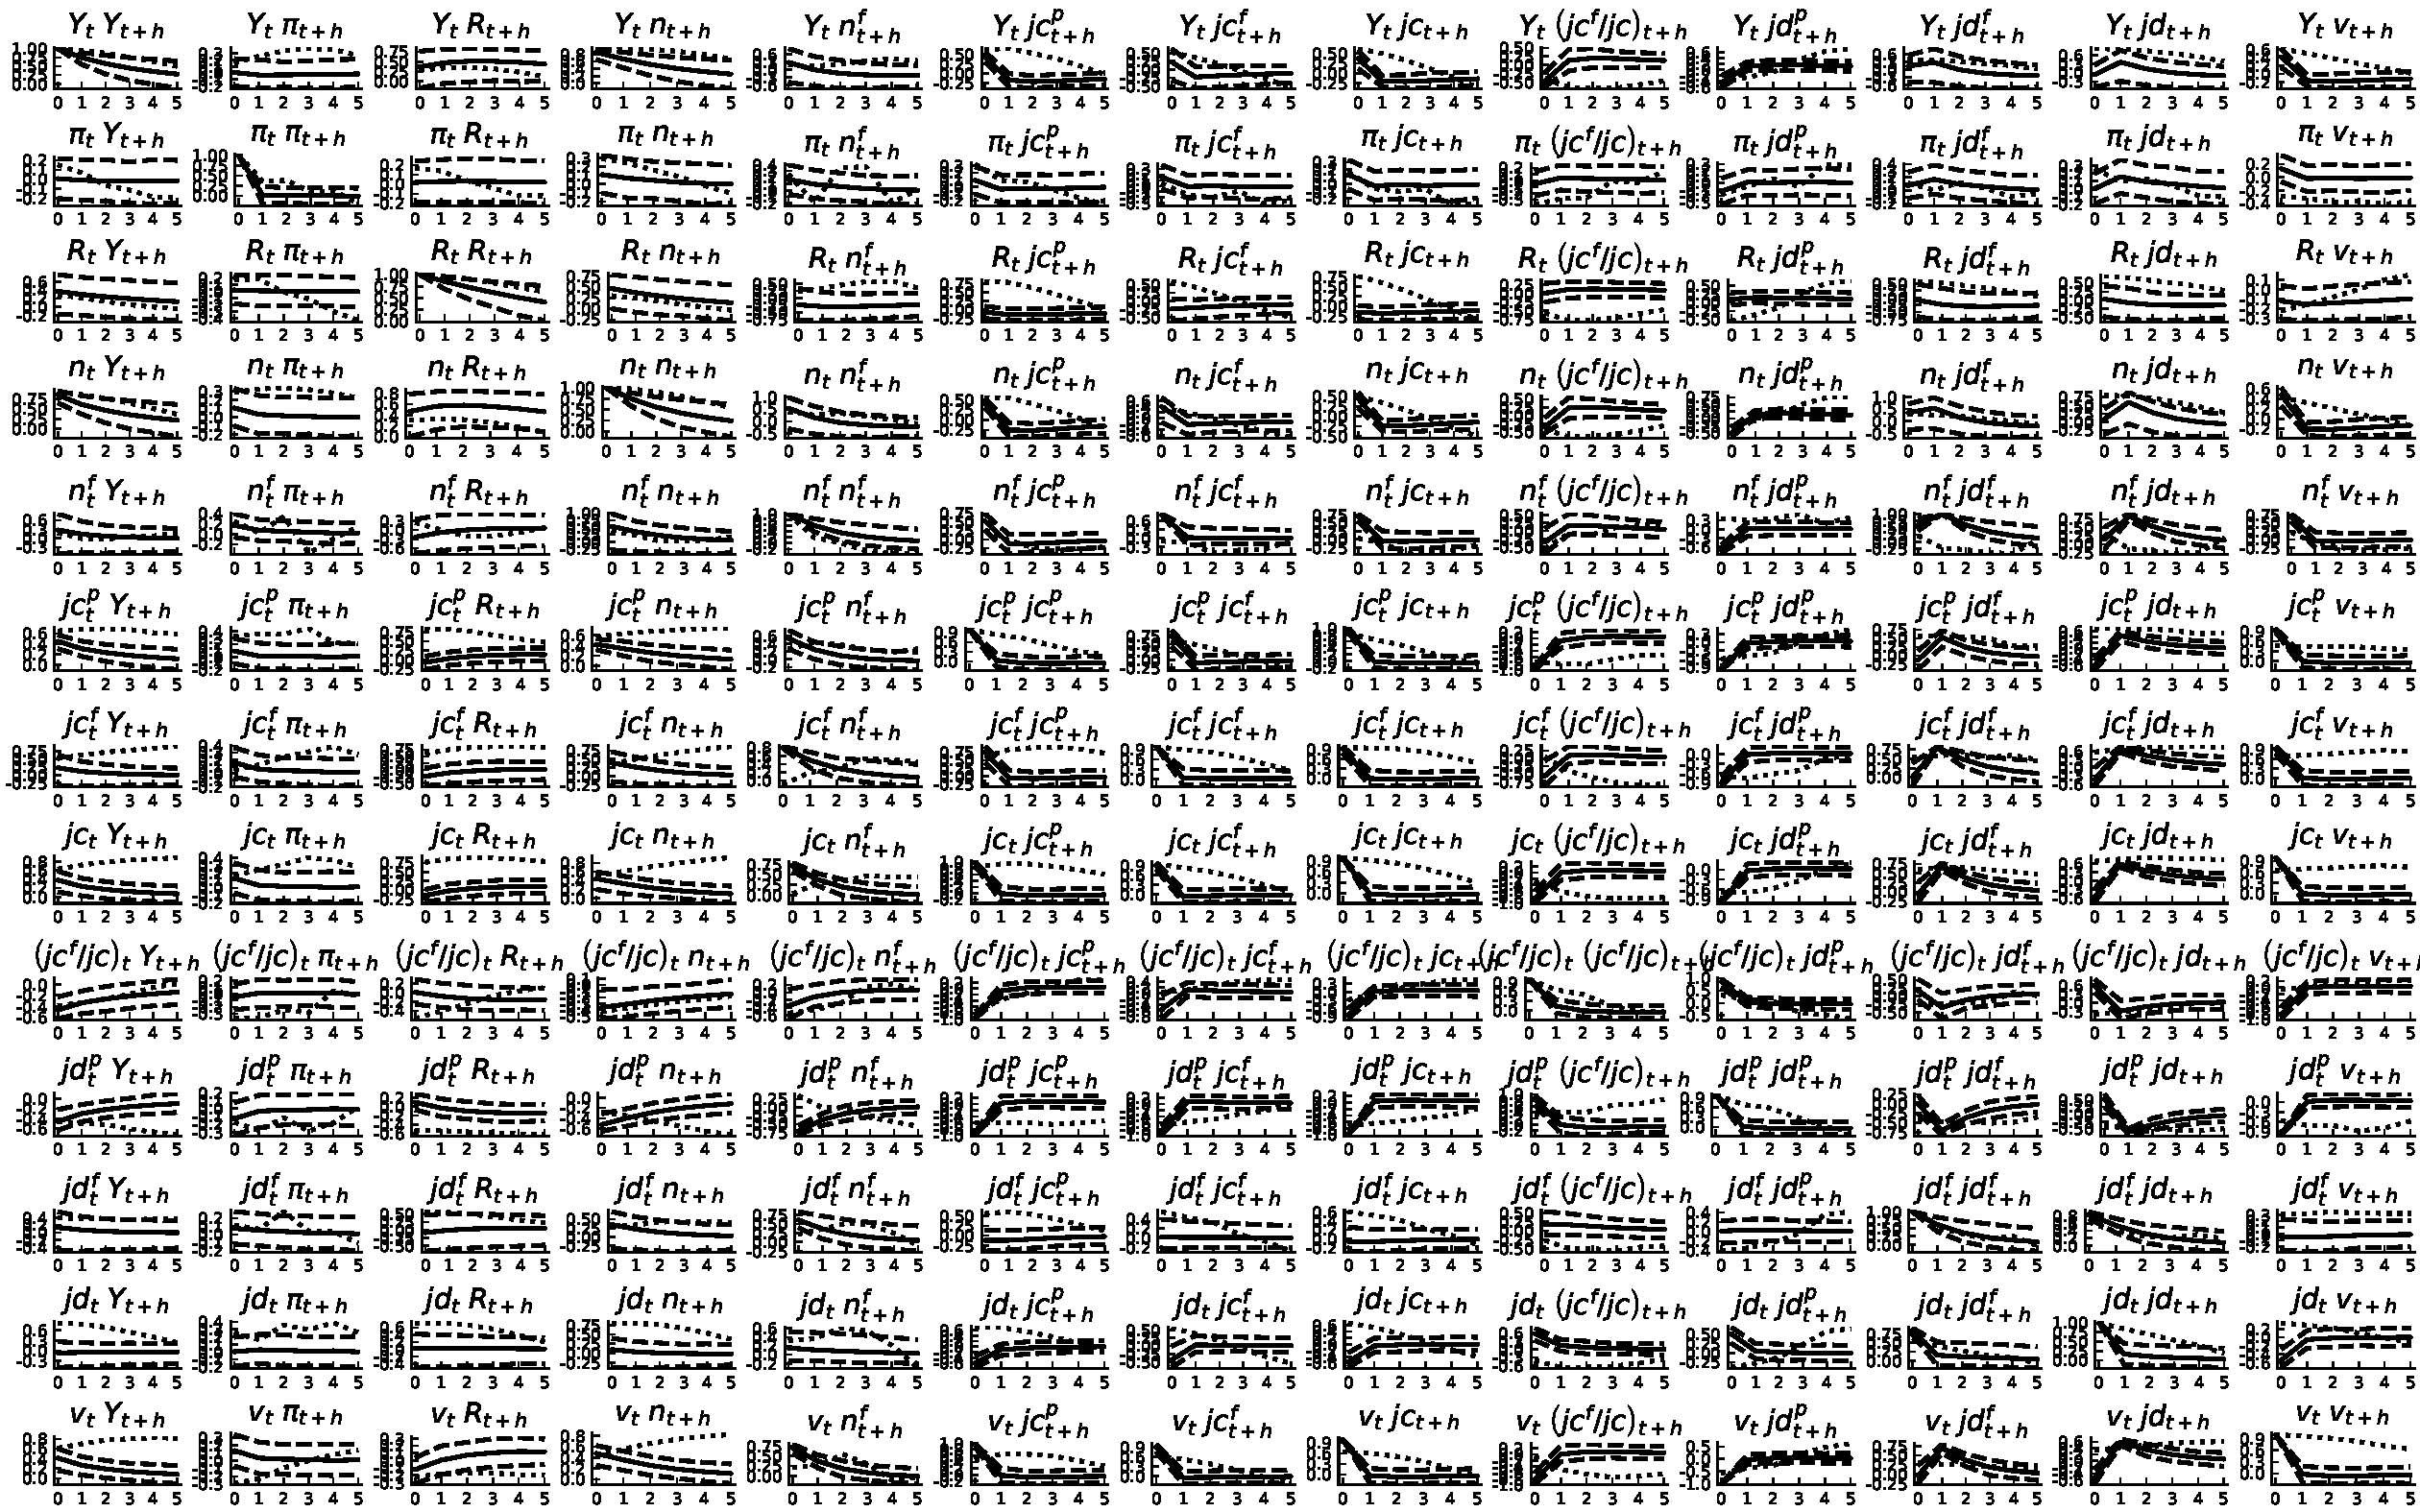
\includegraphics[scale=0.5]{autocor.pdf}
\caption{Simulated and data cross-correlations}
\end{center}
\begin{flushleft}
\footnotesize The x-axis is the lag $h$ and the y-axis is the correlation between the variable $x_t$ and the variable $x_{t+h}$. The solid line is the simulated value, the dashed line is the 95 \% confidence interval around the latter and the dotted line is the value from the data.
\end{flushleft}
\end{figure}

\begin{figure}[H]
\begin{center}
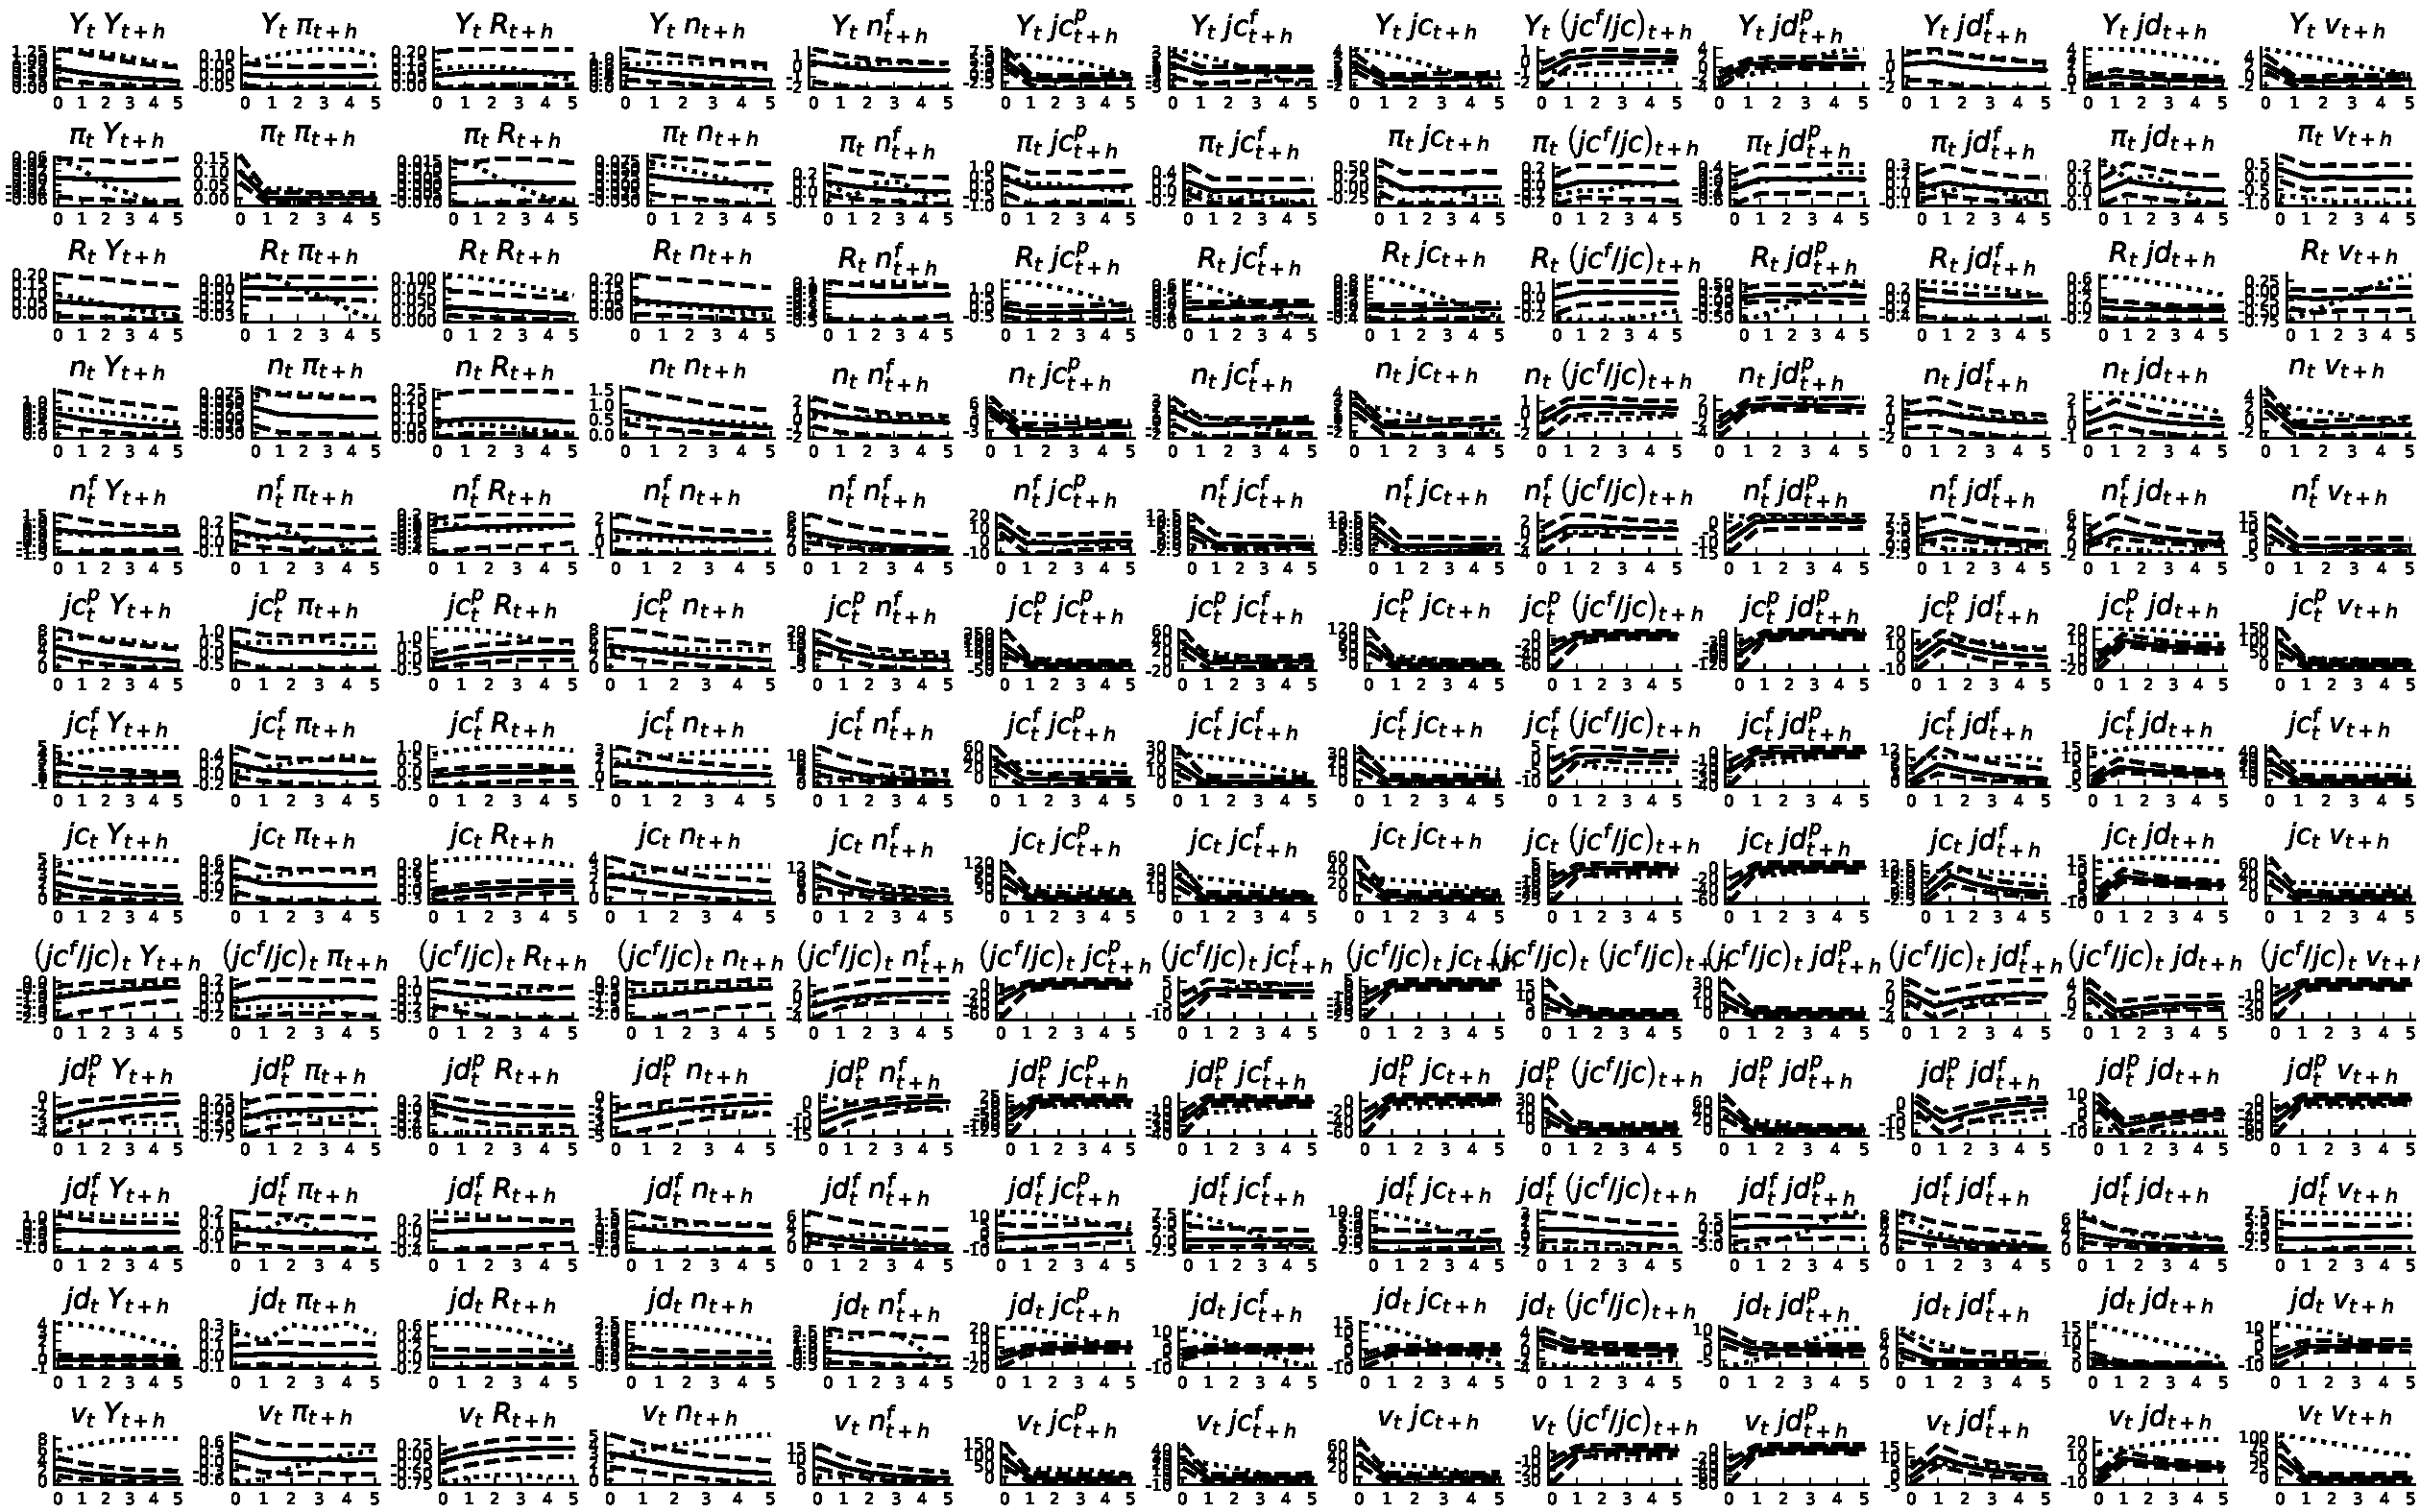
\includegraphics[scale=0.5]{autocov.pdf}
\caption{Simulated and data cross-covariances}
\end{center}
\begin{flushleft}
\footnotesize The x-axis is the lag $h$ and the y-axis is the covariance between the variable $x_t$ and the variable $x_{t+h}$. The solid line is the simulated value, the dashed line is the 95 \% confidence interval around the latter and the dotted line is the value from the data.
\end{flushleft}
\end{figure}
\end{landscape}